\section{Multidimensional Conditioning Approximations}

\subsection{Quasi Monte Carlo Method}

\begin{frame}{Quasi Monte Carlo Method}
\begin{itemize}
	\item MonteCarlo Error bound : $O(N^{-1/2})$ for monte carlo(MC) method
	\item \citet{genz2009computation} claimed independent sample points is the reason of slow convergence.
	\item Via employing low discrepancy sets for sequence, QMC is asymptotically efficient than MC.
	\item With $\boldsymbol{\Delta}\sim U[0,1]^n$,
	$$L_N=\{\mathbf{z}+\boldsymbol{\Delta}\text{ mod }1:\mathbf{z}\in K_N\}$$
	$$K_N=\{i\mathbf{q}\text{ mod }1,i=1,\cdots,N\}$$
	where $\mathbf{q}=\sqrt{\mathbf{p}}$ and $\mathbf{p}$ is set of prime numbers.
	\item Since square root of prime numbers is irrational and linear independent over the rational numbers, 
\end{itemize}
\end{frame}

\begin{frame}{Quasi Monte Carlo Method}
\begin{figure}[ht]
	\centering
	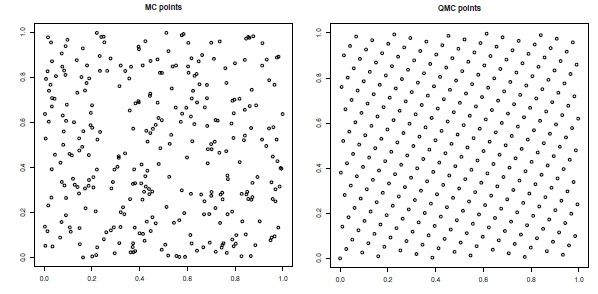
\includegraphics[width=\linewidth]{figs/QMC.jpg}
	\caption{Comparison of MC and QMC sample points\citep{genz2009computation}}
	\label{fig:QMC}
\end{figure}
\end{frame}

\begin{frame}{Quasi Monte Carlo Method}
\footnotesize
\begin{align}
\boldsymbol{\Phi}_n(\mathbf{a}\leq\mathbf{x}\leq\mathbf{b};\boldsymbol{\Sigma})
&=\boldsymbol{\Phi}_n(a\leq\mathbf{Ly}\leq\mathbf{b};I_n)\nonumber\\
&=\int_{a_1\leq l_{11}y_1\leq b_1}\phi(y_1)\cdots\int_{a_n\leq\mathbf{l}_n^t\mathbf{y}\leq b_n}\phi(y_n)d\mathbf{y}\nonumber\\
&=\int_{\tilde{a}_1}^{\tilde{b}_1}\phi(y_1)
\int_{\tilde{a}_2(y_1)}^{\tilde{b}_2(y_1)}\phi(y_2)\cdots
\int_{\tilde{a}_n(y_1,\cdots,y_{n-1})}^{\tilde{b}_n(y_1,\cdots,y_{n-1})}\phi(y_n)d\mathbf{y}\nonumber\\
\text{with } & \tilde{a}_i(y_1,\cdots,y_{i-1})=\frac{a_i-\sum_{j=1}^{i-1}l_{ij}y_j}{l_{ii}}\nonumber\\\text{ and }
&(\tilde{b}_i(y_1,\cdots,y_{i-1}))=\frac{b_i-\sum_{j=1}^{i-1}l_{ij}y_j}{l_{ii}}\nonumber\\
&=\int_{\Phi(\tilde{a}_1)}^{\Phi(\tilde{b}_1)}
\int_{\Phi(\tilde{a}_2(\Phi^{-1}(z_1)))}^{\Phi(\tilde{b}_2(\Phi^{-1}(z_1)))}\cdots
\int_{\Phi(\tilde{a}_n(\Phi^{-1}(z_1),\cdots,\Phi^{-1}(z_{n-1})))}^{\Phi(\tilde{b}_n(\Phi^{-1}(z_1),\cdots,\Phi^{-1}(z_{n-1})))}
d\mathbf{z}(y_i=\Phi^{-1}(z_i))\nonumber\nonumber\\
&=(e_1-d_1)\int_0^1(e_2(w_1)-d_2(w_1))\cdots\nonumber\\
&\int_0^1(e_n(w_1,\cdots,w_{n-1}) - d_n(w_1,\cdots,w_{n-1})))\int_0^1d\mathbf{w}\nonumber\\
\text{with } & z_i=d_i+(e_i-d_i)w_i 
\label{eqn:qmc}
\end{align}
\end{frame}

\begin{frame}{Quasi Monte Carlo Method}
\begin{algorithm}[ht]
	\caption{Multivariate Normal Probability with Quasi Monte Carlo Method}
	\begin{algorithmic}[1]
		\tiny
		\Procedure{\texttt{MVN}}{$\boldsymbol{\mu}, \boldsymbol{\Sigma}, \mathbf{a}, \mathbf{b}, ns, N$}
		\State $\mathbf{L}=\text{cholesky}(\boldsymbol{\Sigma})$
		\State $\mathbf{a}=\mathbf{a}-\boldsymbol{\mu}$; $\mathbf{b}=\mathbf{b}-\boldsymbol{\mu}$
		\State $T=0,N=0,V=0$
		\State $\mathbf{p}$ = vector of primes less than $\frac{5n\log{n+1}}{4}$;$\mathbf{q}=\sqrt{\mathbf{p}}$
		\State $\mathbf{P}=\mathbf{1}_{ns}$
		\State $ans = 0$
		\For{$i=1,\cdots,ns$}
		\State $I_i=0$, $\boldsymbol{\Delta}\sim U(0,1)^n$
		\For{$j=1,\cdots,N$}
		\State $\mathbf{X}[1:n,j]=(j+1)\mathbf{q}+\boldsymbol{\Delta}$
		\State $\mathbf{X}[1:n,j]=2\lvert\mathbf{X}[1:n,j]-\text{floor}(\mathbf{X}[1:n,j])\rvert-1$
		\EndFor
		\State $\mathbf{sample}=\mathbf{O}_{n,N}$
		\State $\mathbf{s},\mathbf{c},\mathbf{d},\mathbf{dc}, \mathbf{P}=\mathbf{0}_N$
		\For{$j=1, \cdots,n$}
		\If{$j>1$}
		\State $c=\min(1, c + X[j-1,:]\odot dc)$
		\State $\mathbf{sample}[i-1,1:N] = \Phi^{-1}(c)$
		\State $s = \mathbf{sample}[1:i-1,1:N]^TL[1:i-1, i]$
		\EndIf
		\State $\mathbf{P} *= \Phi(\frac{b-s}{L[i,i]}) - \Phi(\frac{a-s}{L[i,i]})$
		\EndFor
		\State $\text{ans} += \text{mean}(\mathbf{P})$
		\EndFor
		\State\Return $\text{ans}/ns$
		\EndProcedure
	\end{algorithmic}\label{alg:QMC}
\end{algorithm}
\end{frame}

\begin{frame}{Conditioning Approximation}
\footnotesize
\citet{mendell1974multifactorial}, \citet{kamakura1989estimation}, and \citet{trinh2015bivariate} exploit Cholesky factors from LDL decomposition rather than dealing with original covariance matrix.
Biviarate example is follow.
$$\boldsymbol{\Sigma} = \begin{pmatrix}
\boldsymbol{\Sigma}_{1,1} & \mathbf{R}^T\\
\mathbf{R} & \hat{\boldsymbol{\Sigma}}
\end{pmatrix}\text{, with } \mathbf{L}=\begin{pmatrix}
\mathbf{I}_{2} & \mathbf{O}\\1:
\mathbf{M} & \mathbf{L}
\end{pmatrix}\text{ and } \mathbf{D}=\begin{pmatrix}
\mathbf{D}_{1} & \mathbf{O}\\
\mathbf{O} & \mathbf{\hat{D}}
\end{pmatrix}$$
,where $\boldsymbol{\Sigma}_{1,1}, \mathbf{D}_{1}$ is a $2\times2$ matrix. From $\mathbf{D}_1=\boldsymbol{\Sigma_{1,1}}$, $\mathbf{M}=\mathbf{R}\mathbf{D}_1^{-1}$, $\mathbf{\hat{D}}=\hat{\boldsymbol{\Sigma}}-\mathbf{M}\mathbf{D}_1\mathbf{M}^T$
\begin{align}\label{eqn:phi_cond-biv}
\boldsymbol{\Phi}_n(\mathbf{a},\mathbf{b};\mathbf{0},\boldsymbol{\Sigma})
&= \frac{1}{\sqrt{\lvert\mathbf{D}\rvert(2\pi)^n}}\int_{\alpha_1}^{\beta_1}\int_{\alpha_2}^{\beta_2}e^{-\frac{1}{2}\mathbf{x_2}^T\mathbf{D}_1^{-1}\mathbf{x}_2}\nonumber\\
&\cdots \int_{\alpha_{2k-1}}^{\beta_{2k-1}}\int_{\alpha_{2k}}^{\beta_{2k}}e^{-\frac{1}{2}\mathbf{x_{2k}}^T\mathbf{D}_1^{-1}\mathbf{x}_{2k}}
\end{align}
\end{frame}

\begin{frame}{Conditioning Approximation}
\citet{cao2019hierarchical} generalizes bivariate method of \citet{trinh2015bivariate} to $d$-dimensional. Algorithms and details are following.
\begin{algorithm}[ht]
	\caption{LDL decomposition}
	\begin{algorithmic}[1]
		\tiny
		\Procedure{\texttt{LDL}}{$\boldsymbol{\Sigma}$}
		\State $\mathbf{L} \leftarrow \mathbf{I}_m, \mathbf{D} \leftarrow \mathbf{O}_m$
		\For{$i = 1:d:m-d+1$}
		\State $\mathbf{D}[i:i+d-1,i:i+d-1] \leftarrow \boldsymbol{\Sigma}[i:i+d-1,i:i+d-1]$
		\State $\mathbf{L}[i+d:m,i:i+d-1] \leftarrow \boldsymbol{\Sigma}[i+d:m,i:i+d-1]\mathbf{D}^{-1}[i:i+d-1,i:i+d-1]$
		\State $\boldsymbol{\Sigma}[i+d:m,i+d:m]\leftarrow\boldsymbol{\Sigma}[i+d:m,i+d:m]-\mathbf{L}[i+d:m,i:i+d-1] \mathbf{D}^{-1}[i:i+d-1,i:i+d-1] \mathbf{L}[i:i+d-1,i+d:m]$
		\If{$i+d<m$}
		\State $\mathbf{D}[i+d:m,i+d:m] \leftarrow \boldsymbol{\Sigma}[i+d:m,i+d:m]$
		\EndIf
		\EndFor
		\State\Return $\mathbf{L}$ and $\mathbf{D}$
		\EndProcedure
	\end{algorithmic}\label{alg:LDL-d}
\end{algorithm}
\end{frame}

\begin{frame}{Conditioning Approximation}
\footnotesize
When $s=\frac{m}{d}$ is integer, results of Algorithm \ref{alg:LDL-d}, $\mathbf{L}, \mathbf{D}$ can be written as
$$
\mathbf{L} = \begin{pmatrix}
\mathbf{I}_d & \mathbf{O}_d & \cdots &\mathbf{O}_d\\
\mathbf{L}_{2,1} & \ddots & \ddots &\vdots\\
\vdots & \ddots & \mathbf{I}_d & \mathbf{O}_d\\
\mathbf{L}_{s,1} & \cdots & \mathbf{L}_{s,s-1} &\mathbf{I}_d\\
\end{pmatrix},
\mathbf{D} = \begin{pmatrix}
\mathbf{D}_1 & \mathbf{O}_d & \cdots &\mathbf{O}_d\\
\mathbf{O}_{d} & \ddots & \ddots &\vdots\\
\vdots & \ddots & \mathbf{D}_{s-1} & \mathbf{O}_d\\
\mathbf{O}_d & \cdots & \mathbf{O}_d &\mathbf{D}_s\\
\end{pmatrix}
$$
with $d$-dimensional identitiy matrix $\mathbf{I}_d$ and $d$-dimensional zero matrix $\mathbf{O}_d$ and $d$-dimensional positive-definite matrix $\mathbf{D}_1,\cdots,\mathbf{D}_s$. 
As in \eqref{eqn:phi_cond-biv}, tranformation, $Y=LX$ provides $m$-dimensional multivariate normal prabability as the product of s $d$-dimensional multivariate normal probabilities as below.
\begin{equation}\label{eqn::phi_cond-ddim}
\boldsymbol{\Phi_m}(\mathbf{a},\mathbf{b};\mathbf{0},\boldsymbol{\Sigma})=\int_{\mathbf{\alpha}_1}^{\mathbf{\beta}_1}\phi_d(\mathbf{y}_1;\mathbf{D}_1)\int_{\mathbf{\alpha}_2}^{\mathbf{\beta}_2}\phi_d(\mathbf{y}_2;\mathbf{D}_2)\cdots\int_{\mathbf{\alpha}_s}^{\mathbf{\beta}_s}\phi_d(\mathbf{y}_s;\mathbf{D}_s)d\mathbf{y}_s\cdots d\mathbf{y}_2d\mathbf{y}_1
\end{equation}
,where $\boldsymbol{\alpha}_i=\mathbf{a}_i-\sum_{j=1}^{i-1}\mathbf{L}_{ij}\mathbf{y}_j, \boldsymbol{\beta}_i=\mathbf{b}_i-\sum_{j=1}^{i-1}\mathbf{L}_{ij}\mathbf{y}_j$
\end{frame}

\begin{frame}{Conditioning Approximation}
\begin{algorithm}[ht]
	\caption{d-dimensional conditioning algorithm}
	\begin{algorithmic}[1]
		\footnotesize
		\Procedure{\texttt{CMVN}}{$\boldsymbol{\Sigma},\mathbf{a},\mathbf{b},d$}
		\State $\mathbf{y}\leftarrow\mathbf{0},P\leftarrow1$
		\For{$i = 1:s$}
		\State $j\leftarrow(i-1)d$
		\State $\mathbf{g}\leftarrow\mathbf{L}[j+1:j+d,1:j]\mathbf{y}[1:j]$
		\State $\boldsymbol{\alpha}\leftarrow\mathbf{a}[j+1:j+d]-\mathbf{g}$
		\State $\boldsymbol{\beta}\leftarrow\mathbf{b}[j+1:j+d]-\mathbf{g}$
		\State $\mathbf{D}^\prime\leftarrow\mathbf{D}[j+1:j+d,j+1:j+d]$
		\State $P\leftarrow P\cdot\boldsymbol{\Phi}_d(\boldsymbol{\alpha},\boldsymbol{\beta};\mathbf{0},\mathbf{D}^\prime)$
		\State $\mathbf{y}[j+1:j+d]\leftarrow E[\mathbf{Y}^\prime]$
		\EndFor
		\State\Return $P$ and $\mathbf{y}$
		\EndProcedure
	\end{algorithmic}\label{alg:CMVN}
\end{algorithm}
\end{frame}

\begin{frame}{Multidimensional Truncated Expectations}
\footnotesize
The truncated expectation is expressed as
$$E(X^{e_j})=\frac{1}{\boldsymbol{\Phi}(\mathbf{a},\mathbf{b};\boldsymbol{\mu},\boldsymbol{\Sigma})}\int_\mathbf{a}^\mathbf{b}x_j\phi_d(\mathbf{x};\boldsymbol{\mu},\boldsymbol{\Sigma})d\mathbf{x}=\frac{1}{\boldsymbol{\Phi}(\mathbf{a},\mathbf{b};\boldsymbol{\mu},\boldsymbol{\Sigma})}F_j^d(\mathbf{a},\mathbf{b};\boldsymbol{\mu},\boldsymbol{\Sigma})$$

\begin{theorem}\citep{kan2017moments}
	\label{thm:thmkan}
	$$F_j^d(\mathbf{a},\mathbf{b};\boldsymbol{\mu},\boldsymbol{\Sigma})= \mu_j\boldsymbol{\Phi}_d(\mathbf{a},\mathbf{b};\boldsymbol{\mu},\boldsymbol{\Sigma})+\mathbf{e}_j^T\boldsymbol{\Sigma}\mathbf{c}$$
	,where $c$ is a vector with lth component defined as
	$$\begin{aligned}
	c_l&=\phi_1(a_l;\mu_l,\sigma_l^2)\Phi_{d-1}(\mathbf{a}_{-l},\mathbf{b}_{-l};\boldsymbol{\hat{\mu}}^1, \hat{\boldsymbol{\Sigma}}_l)
	-\phi_1(b_l;\mu_l,\sigma_l^2)\Phi_{d-1}(\mathbf{a}_{-l},\mathbf{b}_{-l};\boldsymbol{\hat{\mu}}^2, \hat{\boldsymbol{\Sigma}}_l)\\
	\boldsymbol{\hat{\mu}}^1_l&=\mu_{-l}+\boldsymbol{\Sigma}_{-l,l}\frac{a_l-\mu_l}{\sigma_l^2},
	\boldsymbol{\hat{\mu}}^2_l=\mu_{-l}+\boldsymbol{\Sigma}_{-l,l}\frac{b_l-\mu_l}{\sigma_l^2},\\
	\hat{\boldsymbol{\Sigma}}_l&=\boldsymbol{\Sigma}_{-l,-l} -\frac{1}{\sigma_l^2}\boldsymbol{\Sigma}_{-l,l}\boldsymbol{\Sigma}_{l,-l}
	\end{aligned}$$
\end{theorem}
Theorem \ref{thm:thmkan} has same form with bivariate version of \citet{trinh2015bivariate} with $d=2$ and it allows us to calculate $E[Y^\prime]$ in Algorithm \ref{alg:CMVN} with $\boldsymbol{\Phi}$ which can be obtained with quasi monte calro method proposed by \citet{genz1992numerical}
\end{frame}

\begin{frame}{Multidimensional Conditioning Approximation with Univariate Reordering}
\footnotesize
Appropriate integration order on conditioning algorithm possibly improves estiation accuracy
\begin{itemize}
	\item \citet{schervish1984algorithm} : integral with shortest integration interval widths be the outermost integration variables
	\item \citet{gibson1994monte} : variables which have smallest expected values be the outermost integration variables.\\
	Since innermost integrals which have smaller variation have the most influence with this order, overall variance reduces.
	\item \citet{trinh2015bivariate} also employs this ordering, and \citet{cao2019hierarchical} generalized it to $d$-dimensional problem.
\end{itemize}
\end{frame}

\begin{frame}{Multidimensional Conditioning Approximation with Univariate Reordering}
\begin{algorithm}[ht]
	\caption{d-dimensional conditioning algorithm with univariate reordering}
	\begin{algorithmic}[1]
		\tiny
		\Procedure{\texttt{RCMVN}}{$\boldsymbol{\Sigma},\mathbf{a},\mathbf{b},d$}
		\State $\mathbf{y}\leftarrow\mathbf{0},\mathbf{C}\leftarrow\boldsymbol{\Sigma}$
		\For{$i = 1:m$}
		\If{$i > 1$}
		\State $\mathbf{y}[i-1]\leftarrow\frac{\phi(a^\prime)-\phi(b^\prime)}{\Phi(b^\prime)-\Phi(a^\prime)}$
		\EndIf
		\State $j\leftarrow\text{argmin}_{i\leq j\leq m}\{\Phi(\frac{\mathbf{b}[j]-\mathbf{C}[j,1:i-1]\mathbf{y}[1:i-1]}{\sqrt{\boldsymbol{\Sigma}[j,j]-\mathbf{C}[j,1:i-1]\mathbf{C}^T[j,1:i-1]}})-\Phi(\frac{\mathbf{a}[j]-\mathbf{C}[j,1:i-1]\mathbf{y}[1:i-1]}{\sqrt{\boldsymbol{\Sigma}[j,j]-\mathbf{C}[j,1:i-1]\mathbf{C}^T[j,1:i-1]}})\}$
		\State $\boldsymbol{\Sigma}[:,(i,j)]\leftarrow\boldsymbol{\Sigma}[:,(j,i)]$;$\boldsymbol{\Sigma}[(i,j),:]\leftarrow\boldsymbol{\Sigma}[(j,i),:]$
		\State $\mathbf{C}[:,(i,j)]\leftarrow\mathbf{C}[:,(j,i)]$;$\mathbf{C}[(i,j),:]\leftarrow\mathbf{C}[(j,i),:]$
		\State $\mathbf{a}[(i,j)]=\mathbf{a}[(j,i)]$
		\State $\mathbf{b}[(i,j)]=\mathbf{b}[(j,i)]$
		\State $\mathbf{C}[i,i]\leftarrow\sqrt{\boldsymbol{\Sigma}[i,i]-\mathbf{C}[i,1:i-1]\mathbf{C}^T[i,1:i-1]}$
		\State $\mathbf{C}[j,i]\leftarrow \frac{\boldsymbol{\Sigma}[j,i]-\mathbf{C}[i,1:i-1]\mathbf{C}^T[j,1:i-1]}{\mathbf{C}[i,i]}$, for $j=i+1,\cdots,m$
		\State $a^\prime=\frac{\mathbf{a}[i]-\mathbf{C}[i,1:i-1]y[1:i-1]}{\mathbf{C[i,i]}}$
		\State $b^\prime=\frac{\mathbf{b}[i]-\mathbf{C}[i,1:i-1]y[1:i-1]}{\mathbf{C[i,i]}}$
		\EndFor
		\State\Return \texttt{CMVN}($\boldsymbol{\Sigma},\mathbf{a},\mathbf{b},d$) as in Algorithm \ref{alg:CMVN}
		\EndProcedure
	\end{algorithmic}\label{alg:RCMVN}
\end{algorithm}

\end{frame}